%%%%%% Krav %%%%%%
\section{Krav}

For at definere systemet er der opstillet en række krav. Aktører til systemet er blevet identificeret og use cases er opstillet for at definere de funktionelle krav. Desuden er der opstillet ikke-funktionelle krav til systemet som helhed og til systemets blokke.\newline

En mere detaljeret beskrivelse af kravene er uddybet i projektets kravspecifikation[x]

\subsection{Funktionelle krav}
Der er defineret 2 aktører i systemet: Bruger \& GPS-satellit.
Bruger er en primær aktør der ønsker at initialisere systemet. Det er bruger der tilslutter de nødvendige moduler til dronen og opretter flyveopsætningen på webapplikationen.
GPS-satellit er en sekundær aktør der giver dronen mulighed for at finde dens egen position. 

På billedet vises aktør diagrammet for systemet. Diagrammet viser hvad aktørerne har fat i eller bruger.
\begin{figure}[H]
	\centering
	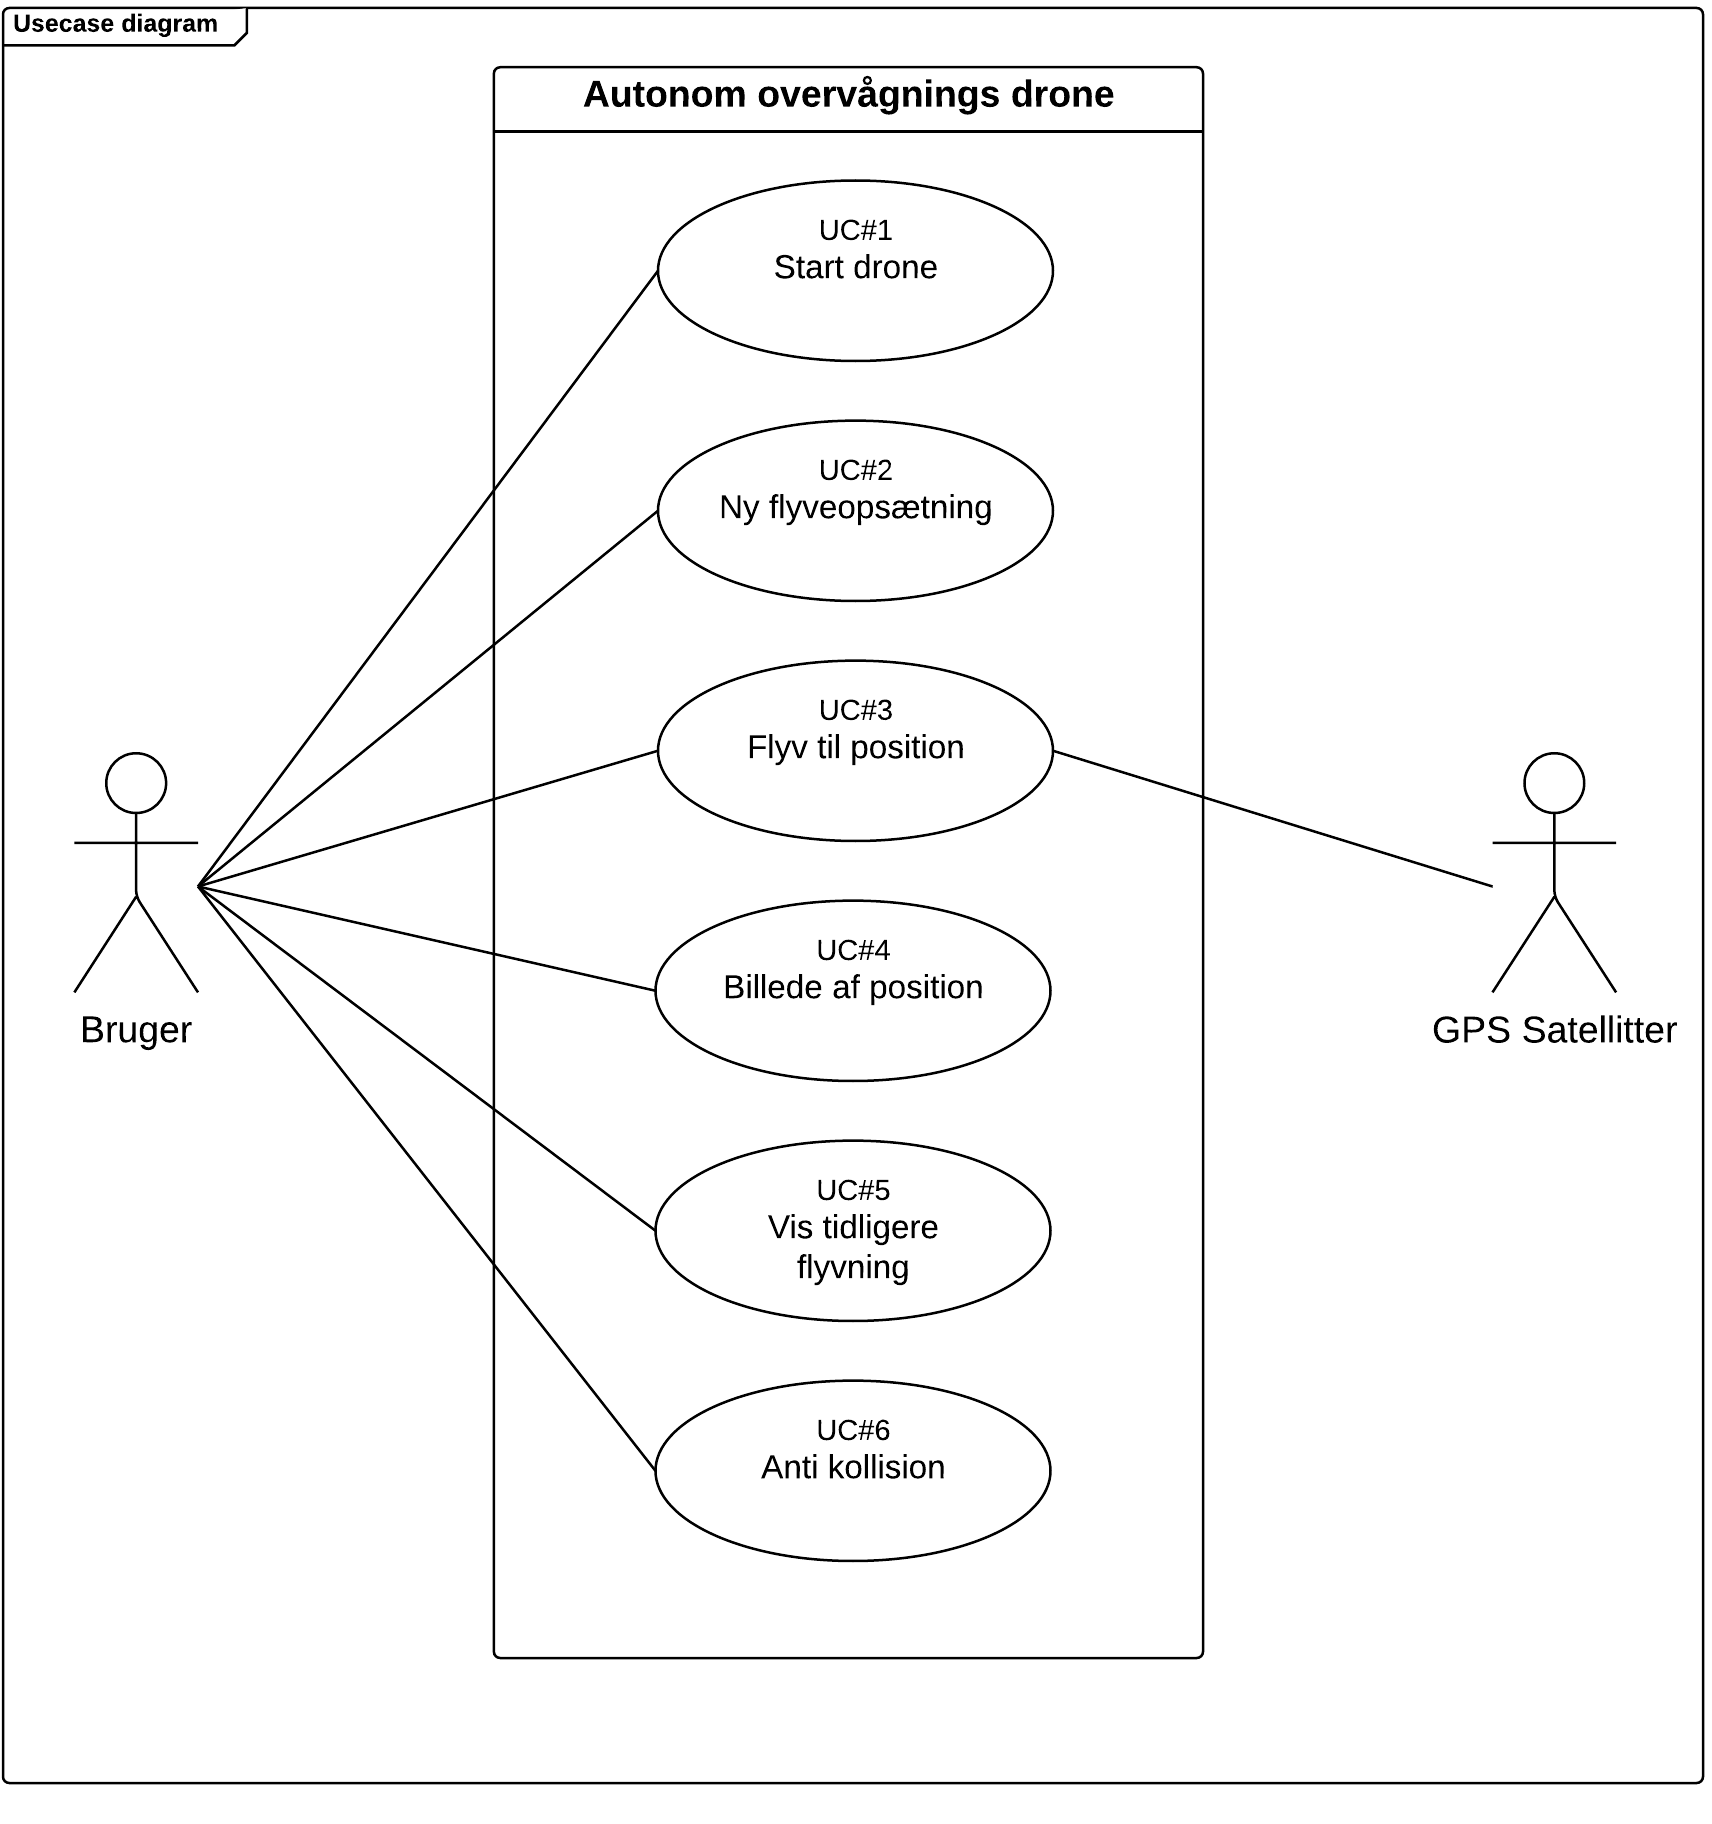
\includegraphics[width=0.60\textwidth]{Billeder/Krav/Use_case_diagram}
	\caption{Use case diagram}
	\label{fig:useCaseDiagram}
\end{figure}

Alle use cases beskrevet i projektets kravspecifikation er specificeret som fully dressed use cases, hvor hovedforløb er successcenariet når use casen er gennemført. \\
Nedenfor vises en beskrivelse af de forskellige use cases og en beskrivelse af deres hovedforløb:

\textbf{Use case 1: Start drone} \\
Bruger tilslutter batteri og dronen initialiseres. Dronen sender dens nuværende position til webapplikationen.\\

\textbf{Use case 2: Ny flyveopsætning} \\
Bruger logger på webapplikation og opretter en ny flyveopsætning. Flyveopsætningen sættes tilgængelig for dronen.\\

\textbf{Use case 3: Flyv til position}\\
Dronen henter flyve opsætningen fra serveren og påbegynder flyvningen. Dronen indstiller sig efter den ønskede flyvehøjde og flyver mod ønsket position. \\

\textbf{Use case 4: Billede af position} \\
Dronen ankommer til den ønskede position og tager et billede. Hvis billedet accepteres, flyver dronen videre mod næste koordinat. \\

\textbf{Use case 5: Vis tidligere flyvninger} \\
Bruger tilgår webapplikationen for at se tidligere flyvninger.\\

\textbf{Use case 6: Anti kollision} \\
Dronens anti kollisions sensorer detekterer et objekt og et undvigningsmanøvre udføres. \\

\newpage
\subsection{Ikke-funktionelle krav}


De ikke-funktionelle krav opstilles ud fra systemspecifikationerne og er krav som ikke kan defineres i use cases. De ikke-funktionelle krav har ingen indvirkning på systemets endelig funktion, kun specifikationerne.
Kravene er grupperet efter hvor i systemet de hører til. 

De generelle krav er krav der omhandler både drone og webapplikation, altså krav der ikke kan placeres i en specifik gruppe.
Derudover er der defineret krav til dronen, da den skal have nogle minimumsværdier eller grænseværdier.
For at sikre at dronen hele tiden er opdateret med information, er der sat krav af til de forskellige sensorer og moduler der samler information ind. 

